\documentclass[11pt]{article}

\usepackage[margin=1in]{geometry}
\usepackage{amsmath,amssymb,amsthm,mathtools,bm}
\usepackage{booktabs,longtable,array,multirow,tabularx}
\usepackage{enumitem}
\usepackage{xcolor}
\usepackage{hyperref}
\usepackage{microtype}
\usepackage{caption}
\usepackage{subcaption}
\usepackage{placeins}
\usepackage{graphicx}
\usepackage{tikz}
\usetikzlibrary{arrows.meta,positioning,calc,fit,shapes.geometric}

\hypersetup{colorlinks=true,linkcolor=blue!50!black,citecolor=blue!50!black,urlcolor=blue!50!black}

\newtheorem{theorem}{Theorem}[section]
\newtheorem{proposition}[theorem]{Proposition}
\newtheorem{lemma}[theorem]{Lemma}
\newtheorem{corollary}[theorem]{Corollary}
\newtheorem{assumption}[theorem]{Assumption}
\theoremstyle{definition}
\newtheorem{definition}[theorem]{Definition}
\theoremstyle{remark}
\newtheorem{remark}[theorem]{Remark}

\newcommand{\R}{\mathbb{R}}
\newcommand{\one}{\mathbf{1}}
\newcommand{\diag}{\operatorname{diag}}
\newcommand{\argmin}{\operatorname*{arg\,min}}
\newcommand{\E}{\mathbb{E}}
\newcommand{\Var}{\operatorname{Var}}
\newcommand{\Cov}{\operatorname{Cov}}
\newcommand{\Tr}{\operatorname{Tr}}
\newcommand{\calF}{\mathcal{F}}
\newcommand{\calE}{\mathcal{E}}
\newcommand{\calL}{\mathcal{L}}
\newcommand{\T}{^{\mathsf T}}
\newcommand{\SD}{S_D}

\title{Adaptive Green Risk Fields for Causal Fraud Detection}
\author{Maksim Kosmakov\thanks{Department of Mathematical Sciences, University of Cincinnati,
P.O. Box 210025, Cincinnati, OH 45221, USA. Email: \texttt{maximkosmakov@gmail.com}.}}
\date{}

\begin{document}
\maketitle

\begin{abstract}
Fraud screening on transaction streams is a delayed-feedback graph problem: a deployable score must be computed before the candidate transaction and before any label from that transaction can influence the system. We introduce an adaptive Green risk field that propagates released fraud history over a dynamic transaction graph while weighting each node by the reliability of its local history. The estimator is a graph-Tikhonov minimizer, an implicit message-passing layer, and the posterior mean under a working Gaussian Markov random field model. Its mean-squared-error (MSE) decomposition allows shrinkage-biased released histories and yields a regime criterion comparing the raw-minus-smoothed variance term with the induced change in squared bias. Favorable regimes arise when released histories are noisy and graph-induced bias remains limited. In block-causal experiments on IEEE-CIS, tail-ranking models using Green-risk features improve over raw released history across all tested label-release delays. The standalone graph marginal is positive under immediate release and attenuates as labels are delayed. Leakage audits and label-permutation placebos assess temporal validity and signal provenance; paired block-bootstrap intervals and delay sweeps assess stability; calibration and posterior-uncertainty diagnostics characterize the resulting scores. An Elliptic++ evaluation provides a complementary operating-budget saturation case consistent with the regime criterion. The resulting layer is interpretable and temporally auditable, with features designed for fraud-alert ranking under delayed labels.
\end{abstract}

\noindent\textbf{Keywords:} fraud detection; dynamic graphs; delayed feedback; temporal leakage; graph Laplacian; label propagation; risk ranking

\vspace{0.75em}

\section{Introduction and positioning}

Fraud detection is commonly benchmarked as supervised classification, but deployment is a chronological decision problem. A production score may depend only on transactions, graph structure, and labels available before the candidate transaction is evaluated. This constraint matters because fraud risk is associated with identifiers that recur over time--cards, devices, email domains, accounts, addresses, merchants, and wallets--while labels may arrive after a substantial delay and several transactions may share the same recorded timestamp. A graph-based risk layer must therefore combine relational information with an explicit account of what was observable at scoring time.

The proposed layer starts from \emph{released history}. For an entity node $v$, $H_v$ is a causal estimate of its fraud rate formed only from labels released before scoring. Such an estimate is stable for repeatedly observed entities and noisy for new or sparsely observed entities. The adaptive Green field
\begin{equation}
        S_D=(L+D)^{-1}DH,
        \label{eq:main-field}
\end{equation}
combines the historical graph Laplacian $L$ with the diagonal history-fidelity matrix $D=\diag(d_v)$. The inverse $(L+D)^{-1}$ is the Green operator for the regularized graph system, and $DH$ is its source term. A large $d_v$ keeps $(S_D)_v$ close to the local estimate $H_v$; a small $d_v$ allows neighboring histories to have greater influence.

The construction is rooted in established methods for graph regularization and label propagation, where Laplacian energies extend sparse information over weighted graphs \cite{zhu2003,zhou2004,belkin2006,smola2003,chapelle2006}. Its probabilistic interpretation uses Gaussian Markov random fields and graph-smooth precision operators \cite{rueheld,chung1997,rasmussen2006}, while the signal-processing interpretation follows the graph-filtering viewpoint \cite{shuman2013,ortega2018}. These connections provide the variational, averaging, uncertainty, and message-passing descriptions developed in Section~\ref{sec:theory}.

Fraud detection introduces additional constraints: severe class imbalance, delayed feedback, fixed investigation budgets, and evolving relational structure \cite{boltonhand2002,phua2010,davis2006relationship,saito2015precision,akoglu2015,ranshous2015}. Recent graph and temporal-network models motivate richer representations of financial interactions \cite{weber2019,elmougy2023,kipf2017,hamilton2017,velickovic2018,pareja2020,sankar2020,xu2020,rossi2020}. The present study focuses on a narrower object: an auditable released-history layer whose graph state, label set, and inputs are fixed at each scoring time.

The main theoretical result is an MSE decomposition for the adaptive field that includes the regularization bias already present in the released-history estimator. It separates the change in squared bias caused by graph smoothing from the corresponding change in estimator variance. This gives the paper's regime criterion: graph smoothing reduces MSE when the raw-minus-smoothed variance term exceeds the induced change in squared bias. The experiments test that criterion under timestamp-block causality. On IEEE-CIS, tail-ranking models using Green-risk features improve over raw released history across all tested release delays, whereas the standalone smoothing marginal is concentrated near immediate release. Elliptic++ provides a complementary operating-budget saturation case in which released address history already saturates the top alert budget and local Green smoothing adds no further benefit. Calibration is evaluated separately from alert ranking because calibrated probabilities and top-budget orderings serve different operational purposes \cite{zadrozny2002,niculescu2005,guo2017}.

\section{Notation and causal transaction graph}
\label{sec:causal-setting}

Let transactions be indexed in chronological order by $i$. Transaction $i$ has feature vector $x_i$, observed timestamp $\tau_i$, binary fraud label $Y_i\in\{0,1\}$, and label-release time $\rho_i$. The label may be used only after $\rho_i$. To \emph{score} transaction $i$ means to compute a risk score $q_i$ before inserting any edge generated by $x_i$ or any label information associated with it.

For a recorded timestamp $t$, let $\calF_{t^-}$ denote the information available immediately before the transactions at time $t$ are scored:
\[
    \calF_{t^-}
    =\sigma\!\left(\{x_i:\tau_i<t\},\;\{\text{edges inserted before }t\},\;\{Y_i:\rho_i<t\}\right).
\]
For a candidate transaction $i$ with $\tau_i=t$, define the candidate-specific scoring information set
\[
    \mathcal I_i:=\calF_{t^-}\vee\sigma(x_i).
\]
Accordingly, $q_i$ is required to be $\mathcal I_i$-measurable: it may use the candidate's observed attributes and the frozen historical state, but not candidate-generated graph edges, the candidate label, or information from other transactions in the same timestamp block.

The graph nodes are reusable transaction entities, such as cards, devices, email domains, accounts, addresses, merchants, or wallets. For each relation type $r$, the historical graph at time $t^-$ is
\[
    G_{t^-}^{(r)}=(V_{t^-},E_{t^-}^{(r)},W_{t^-}^{(r)}),
\]
where $V_{t^-}$ is the set of entities already observed, $E_{t^-}^{(r)}$ is the support of the relation-$r$ edges already inserted, and $W_{t^-}^{(r)}$ is the nonnegative weighted adjacency matrix. The edge weight $W_{uv,t^-}^{(r)}$ records the chosen causal strength of relation $r$ between entities $u$ and $v$, such as co-occurrence frequency, recency-weighted frequency, or relation strength computed from earlier transactions. The corresponding weighted-degree matrix has diagonal entries
\[
    (\Delta_{W,t^-}^{(r)})_{vv}=\sum_u W_{vu,t^-}^{(r)},
\]
so the combinatorial Laplacian is
\[
    L_{t^-}^{(r)}=\Delta_{W,t^-}^{(r)}-W_{t^-}^{(r)}.
\]
When several relation graphs are used, they may be combined as
\begin{equation}
    L_{t^-}=\sum_r \theta_r L_{t^-}^{(r)},\qquad \theta_r\ge 0.
    \label{eq:relation-layers}
\end{equation}
Here $\theta_r$ specifies the relative scale of relation $r$. Such weights are fixed before test scoring and are not updated from labels in the scoring block. A single relation layer corresponds to $\theta_r=1$. In the IEEE-CIS implementation, typed entity nodes are formed from public transaction attributes, and the Green-risk fields are computed separately on four relation layers:
\[
    \texttt{card1--addr1},\quad
    \texttt{card1--P\_emaildomain},\quad
    \texttt{card1--DeviceInfo},\quad
    \texttt{DeviceInfo--P\_emaildomain}.
\]
An edge is created only when both endpoint fields are observed; missing or empty values are excluded rather than represented as shared ``missing'' nodes. Each prior transaction contributes unit co-occurrence weight to each available layer edge, and each selected layer is solved with $\theta_r=1$ rather than tuning a summed multi-layer Laplacian. Layer-specific endpoint fields and aggregate summaries are then supplied to the ranking models. In the remainder, $L$ denotes either one layer or a fixed sum of this form. We reserve $D$ for history confidence; $\Delta_W$ denotes weighted graph degree.

Candidate edges are withheld until after scoring. If a new entity appears in the candidate transaction, it is temporarily included as an isolated node. Its endpoint features are therefore defined without using the candidate edge itself.

The released-history vector $H$ is built from labels whose release time precedes the scoring time. For node $v$, an \emph{exposure} is a previously scored transaction incident to $v$. Let $n_v$ be the number of such exposures whose labels have been released before scoring, and let $f_v$ be the number labeled as fraud. A convenient shrinkage estimate is
\begin{equation}
    H_v=\frac{f_v+\alpha \bar p}{n_v+\alpha},
    \label{eq:history}
\end{equation}
where $\bar p$ is the causal global fraud rate computed from released labels and $\alpha>0$ is a prior-strength parameter. The confidence matrix
\[
    D=\diag(d_v),\qquad d_v>0,
\]
records the fidelity weight assigned to the local estimate $H_v$. In the experiments we use the concave rule $d_v=d_0+\sqrt{n_v}$, where $d_0>0$ is a separate confidence offset. Thus confidence increases with released evidence, but more slowly than the raw exposure count; the shrinkage strength $\alpha$ in \eqref{eq:history} and the confidence offset $d_0$ play distinct roles. The beta-binomial calculation in Section~\ref{sec:theory} gives a reference precision scale and explains why a tempered rule is useful in sparse fraud data.

\begin{center}
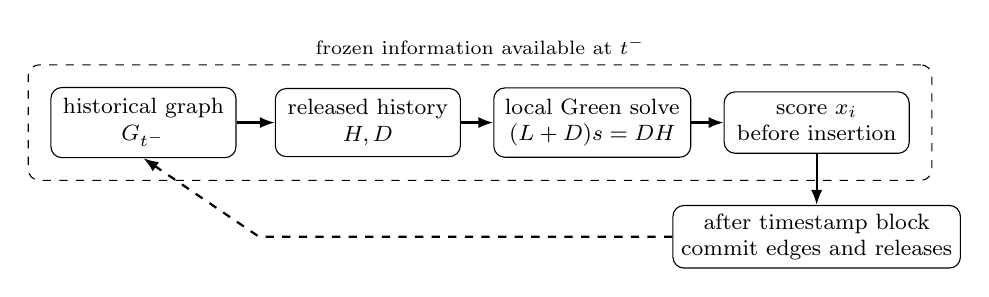
\begin{tikzpicture}[
    font=\footnotesize,
    block/.style={draw,rounded corners,align=center,minimum width=2.35cm,minimum height=0.78cm,inner sep=4pt},
    smallblock/.style={draw,rounded corners,align=center,minimum width=2.35cm,minimum height=0.72cm,inner sep=3pt},
    arrow/.style={-{Latex[length=1.9mm]},thick}
]
\node[block] (past) at (0,0) {historical graph\\$G_{t^-}$};
\node[block] (hist) at (2.85,0) {released history\\$H,D$};
\node[block] (solve) at (5.70,0) {local Green solve\\$(L+D)s=DH$};
\node[block] (score) at (8.55,0) {score $x_i$\\before insertion};
\node[smallblock] (commit) at (8.55,-1.45) {after timestamp block\\commit edges and releases};
\draw[arrow] (past) -- (hist);
\draw[arrow] (hist) -- (solve);
\draw[arrow] (solve) -- (score);
\draw[arrow] (score) -- (commit);
\draw[arrow,dashed] (commit.west) -- ++(-5.25,0) -- (past.south);
\node[draw,dashed,rounded corners,fit=(past)(hist)(solve)(score),inner sep=8pt,label={[font=\scriptsize]above:{frozen information available at $t^-$}}] {};
\end{tikzpicture}
\captionof{figure}{Timestamp-block causal scoring. All transactions with the same timestamp are scored against the same frozen historical state. Candidate edges and labels from that block are committed only after the block has been scored.}
\label{fig:graph}
\end{center}

\section{Adaptive Green smoothing}
\label{sec:theory}

For the theory, fix one causal graph snapshot and suppress time subscripts. The adaptive field is
\[
    \SD=(L+D)^{-1}DH.
\]
Its basic variational form explains the two forces in the estimator: graph smoothness and fidelity to released local history.

\begin{proposition}[Energy minimizer]
Let $L\succeq0$ be the Laplacian of an undirected weighted graph, with each edge in $E$ counted once, and let $D\succ0$ be diagonal. Then $\SD$ is the unique minimizer of
\begin{equation}
    \calE(s)=\frac12\sum_{(u,v)\in E}w_{uv}(s_u-s_v)^2
    +\frac12\sum_{v\in V}d_v(s_v-H_v)^2.
    \label{eq:energy}
\end{equation}
\end{proposition}

\begin{proof}
Since $s^\top Ls=\sum_{(u,v)}w_{uv}(s_u-s_v)^2$, the energy is
\[
    \calE(s)=\frac12s^\top Ls+\frac12(s-H)^\top D(s-H).
\]
The Hessian is $L+D\succ0$, so the minimizer is unique. Stationarity gives $(L+D)s=DH$, hence $s=(L+D)^{-1}DH$.
\end{proof}

The same linear system also gives a maximum principle. Define
\[
    P_D=(L+D)^{-1}D,
\]
so that $S_D=P_DH$.

\begin{lemma}[Convex-combination operator]
The matrix $P_D$ is entrywise nonnegative and satisfies $P_D\one=\one$. Consequently, each component of $S_D=P_DH$ is a convex combination of the entries of $H$.
\end{lemma}

\begin{proof}
Because $L\one=0$, $(L+D)\one=D\one$, and hence $P_D\one=\one$. To prove nonnegativity, let $h\ge0$ componentwise and let $s=P_Dh$, so $(L+D)s=Dh$. If $s_v<0$ were a minimum component of $s$, then
\[
    (Ls)_v=\sum_u w_{vu}(s_v-s_u)\le0
\]
and therefore $((L+D)s)_v=(Ls)_v+d_vs_v<0$, whereas $(Dh)_v=d_vh_v\ge0$. This contradiction shows that $P_Dh\ge0$ whenever $h\ge0$, which is equivalent to entrywise nonnegativity of $P_D$.
\end{proof}

\begin{corollary}[Maximum principle and non-expansiveness]
If $m\le H_v\le M$ for all $v$, then
\[
    m\le (S_D)_v\le M\qquad \forall v.
\]
Moreover, for any histories $H,\widetilde H$,
\[
    \|P_DH-P_D\widetilde H\|_\infty\le \|H-\widetilde H\|_\infty.
\]
\end{corollary}

\begin{proof}
Each row of $P_D$ is nonnegative and sums to one, so applying it preserves componentwise bounds. The same row-sum property gives $\|P_D\|_{\infty}=1$, which yields the stated Lipschitz bound.
\end{proof}

Thus smoothing cannot create scores outside the range of the released histories, and perturbations of those histories are not amplified in the sup norm.

Writing $L=\Delta_W-W$ turns the optimality equation into the nodewise fixed point
\begin{equation}
    (\SD)_v=\frac{d_vH_v+\sum_{u\sim v}w_{uv}(\SD)_u}{d_v+\sum_{u\sim v}w_{uv}}.
    \label{eq:nodewise}
\end{equation}
Thus $d_v$ is the local-history fidelity weight assigned to node $v$. When $d_v$ is large compared with the weighted degree of $v$, the score is anchored near $H_v$; when $d_v$ is small, the score moves toward a weighted neighborhood average. This gives an implicit message-passing layer with a closed-form linear solve.

Local computation follows from the same linear algebra. Let $A=L+D$, and partition the nodes into a retained local set $B$ and a complementary set $I$:
\[
    A=\begin{pmatrix}A_{BB}&A_{BI}\\ A_{IB}&A_{II}\end{pmatrix}.
\]
The Schur complement of $A_{II}$ is
\[
    S_B:=A_{BB}-A_{BI}A_{II}^{-1}A_{IB}.
\]
Eliminating the variables $s_I$ from $As=DH$ gives
\[
    S_Bs_B=(DH)_B-A_{BI}A_{II}^{-1}(DH)_I.
\]
This identity motivates local Green computations: variables outside a retained neighborhood can be eliminated into an effective boundary system. The implementation below instead solves the system directly on each selected radius-2/cap-100 ego graph; the resulting field is exact for that capped local graph.

The field also has a probabilistic interpretation as a working Gaussian Markov random field (GMRF) posterior mean. Consider the graph-smooth prior and heteroskedastic observation model
\[
    p(s)\propto \exp\left(-\frac12s^\top Ls\right),
    \qquad
    H_v\mid s_v\sim N(s_v,d_v^{-1})\quad\text{independently}.
\]

\begin{proposition}[GMRF posterior mean]
The posterior is Gaussian with
\[
    \E[s\mid H]=(L+D)^{-1}DH=\SD,
    \qquad
    \Cov(s\mid H)=(L+D)^{-1}.
\]
\end{proposition}

\begin{proof}
The negative log posterior is, up to constants,
\[
    \frac12s^\top Ls+\frac12(H-s)^\top D(H-s)
    =\frac12s^\top(L+D)s-s^\top DH+\text{const.}
\]
Completing the square gives precision $L+D$, covariance $(L+D)^{-1}$, and mean $(L+D)^{-1}DH$.
\end{proof}

The prior precision $L$ is singular, as in an intrinsic GMRF, but the posterior is proper because $D\succ0$. The posterior covariance gives a per-node uncertainty estimate
\begin{equation}
    \sigma_v^2=[(L+D)^{-1}]_{vv}.
    \label{eq:posterior-var}
\end{equation}
For a transaction with endpoints $a,b$, the corresponding diagnostic features include $\sigma_a$, $\sigma_b$, and standardized contrasts. Using the released global fraud rate $\bar p$ from \eqref{eq:history} as the causal reference level, examples are
\[
    \frac{(S_D)_a-\bar p}{\sigma_a},
    \qquad
    \frac{(S_D)_b-\bar p}{\sigma_b},
    \qquad
    \frac{(S_D)_a-(S_D)_b}{\sqrt{\sigma_a^2+\sigma_b^2}}.
\]

\begin{lemma}[Posterior variance bound]
For every node,
\[
    0<\sigma_v^2\le \frac1{d_v}.
\]
Equality holds for an isolated node.
\end{lemma}

\begin{proof}
Since $L\succeq0$, we have $L+D\succeq D\succ0$. By antitonicity of the inverse on positive definite matrices, $(L+D)^{-1}\preceq D^{-1}$. Taking diagonal entries gives the bound.
\end{proof}

A beta-binomial calculation gives a reference scale for $D$. Let the prior fraud rate at node $v$ be $p_v\sim\operatorname{Beta}(a,b)$. After $n_v$ released exposures, of which $f_v$ are fraudulent, the posterior mean is
\[
    H_v=\frac{a+f_v}{a+b+n_v}.
\]
Equation~\eqref{eq:history} is obtained by taking $a=\alpha\bar p$ and $b=\alpha(1-\bar p)$. The posterior variance is
\[
    \Var(p_v\mid f_v,n_v)=\frac{H_v(1-H_v)}{a+b+n_v+1},
\]
so the inverse-variance scale is
\begin{equation}
    d_v^{\mathrm{BB}}=\frac{a+b+n_v+1}{H_v(1-H_v)}.
    \label{eq:eb-d}
\end{equation}
Because $H_v(1-H_v)$ can be very small in rare-event data, direct use of this precision may assign excessive weight to a few high-count nodes. A capped version is
\begin{equation}
    d_v^{\mathrm{BB,cap}}=\min\left\{d_{\max},\frac{a+b+n_v+1}{\max\{H_v(1-H_v),\epsilon\}}\right\}.
    \label{eq:eb-cap}
\end{equation}
The square-root rule used in the experiments is a tempered alternative: it preserves the ordering by exposure count while limiting the leverage of highly observed hubs.

\section{Bias--variance regime for smoothing}
\label{sec:mse}

The next result gives the regime criterion in a form that matches the shrinkage history used in the experiments. Fix a causal graph snapshot and condition on its released exposure counts. Let $r\in\R^V$ be the latent node-risk vector and write the released-history estimator as
\[
    H=r+b_H+\eta,
    \qquad
    \E\eta=0,
    \qquad
    \Cov(\eta)=\Sigma\succeq0,
\]
where $b_H=\E H-r$ is the bias already introduced by local-history regularization and $\Sigma$ is the covariance of the remaining estimation noise. The raw estimator is $H$ and the smoothed estimator is $P_DH$, where $P_D=(L+D)^{-1}D$. For any estimator $\widehat r$, define
\[
    \operatorname{MSE}(\widehat r):=\E\|\widehat r-r\|_2^2.
\]

\begin{theorem}[MSE decomposition with shrinkage-biased histories]
\label{thm:mse-decomp}
Under the model above,
\begin{align}
    \operatorname{MSE}(P_DH)-\operatorname{MSE}(H)
    &={\underbrace{\bigl\|(P_D-I)r+P_Db_H\bigr\|_2^2-\|b_H\|_2^2}_{\text{change in squared bias}}}
    \notag\\[-0.25em]
    &\quad-{\underbrace{\Tr\!\left(\Sigma-P_D\Sigma P_D^\top\right)}_{\text{raw-minus-smoothed variance}}}.
    \label{eq:mse-decomp}
\end{align}
Consequently, smoothing reduces MSE exactly when
$\Tr(\Sigma-P_D\Sigma P_D^\top)$ exceeds the change in squared bias. When $b_H=0$, the bias term reduces to $\|(P_D-I)r\|_2^2$, the graph-smoothing bias from the unbiased-history model. Under the matched-noise specialization $\Sigma=D^{-1}$, the variance-reduction term is nonnegative.
\end{theorem}

\begin{proof}
The raw history has bias $b_H$ and covariance $\Sigma$, so
\[
    \operatorname{MSE}(H)=\|b_H\|_2^2+\Tr(\Sigma).
\]
The smoothed estimator has bias
\[
    \E[P_DH]-r=(P_D-I)r+P_Db_H,
\]
and covariance $P_D\Sigma P_D^\top$. Subtracting the two bias--variance decompositions gives \eqref{eq:mse-decomp}. Under $\Sigma=D^{-1}$, set $B=D^{-1/2}LD^{-1/2}\succeq0$. Then
\[
    P_DD^{-1}P_D^\top
    =D^{-1/2}(I+B)^{-2}D^{-1/2}\preceq D^{-1},
\]
because every eigenvalue of $(I+B)^{-2}$ lies in $(0,1]$.
\end{proof}

The bias vector in Theorem~\ref{thm:mse-decomp} can be written explicitly for the released-history estimator used in the experiments. Let
\[
    A_\alpha=\diag\!\left(\frac{n_v}{n_v+\alpha}\right).
\]
Conditional on the exposure counts and treating the causal global rate $\bar p$ as the current reference value, suppose $\E[f_v\mid n_v,r_v]=n_vr_v$. Then
\[
    \E[H\mid n,r,\bar p]
    =A_\alpha r+(I-A_\alpha)\bar p\one,
\]
so the shrinkage bias is
\begin{equation}
    b_H=(I-A_\alpha)(\bar p\one-r),
    \qquad
    (b_H)_v=\frac{\alpha}{n_v+\alpha}(\bar p-r_v).
    \label{eq:shrinkage-bias}
\end{equation}
Thus the regularization bias is concentrated at nodes with little released history and vanishes as $n_v$ grows. Under an independent conditional-binomial approximation,
\begin{equation}
    \Sigma_{vv}=\frac{n_vr_v(1-r_v)}{(n_v+\alpha)^2},
    \qquad
    \Sigma_{uv}=0\quad(u\ne v).
    \label{eq:shrinkage-cov}
\end{equation}
The theorem does not require this diagonal approximation: shared transactions, the estimated global reference $\bar p$, and overlapping endpoint histories may produce a non-diagonal $\Sigma$. Likewise, the experimental rule $d_v=d_0+\sqrt{n_v}$ is a tempered confidence weight and need not equal $\Sigma_{vv}^{-1}$.

Equation~\eqref{eq:mse-decomp} gives the regime criterion used throughout the experiments. Smoothing is favored when noisy released histories leave substantial variance to remove, graph neighborhoods are sufficiently aligned with latent risk, and the graph update does not amplify the shrinkage bias in \eqref{eq:shrinkage-bias}. As released histories become more precise, both their sampling variance and their shrinkage bias decrease, leaving less scope for graph smoothing to improve MSE.

\begin{corollary}[High-confidence limit]
\label{cor:high-confidence}
Fix $L$ and $r$. For each $k$, let
\[
    H_k=r+b_{H,k}+\eta_k,
    \qquad \E\eta_k=0,
    \qquad \Cov(\eta_k)=\Sigma_k,
\]
and let $P_k=(L+D_k)^{-1}D_k$, where $D_k\succ0$ and $\lambda_{\min}(D_k)\to\infty$. If
\[
    \sup_k\|b_{H,k}\|_2<\infty,
    \qquad
    \sup_k\Tr(\Sigma_k)<\infty,
\]
then
\[
    \operatorname{MSE}(P_kH_k)-\operatorname{MSE}(H_k)\longrightarrow0.
\]
In particular, the marginal effect of smoothing vanishes when the field assigns increasing fidelity to released histories with bounded second moments.
\end{corollary}

\begin{proof}
Since
\[
    P_k-I=-(L+D_k)^{-1}L,
\]
we have
\[
    \|P_k-I\|_2
    \le \frac{\|L\|_2}{\lambda_{\min}(D_k)}
    \longrightarrow0.
\]
Let $Q_k=P_k-I$. The change in squared bias equals
\[
    2b_{H,k}^\top Q_k(r+b_{H,k})+\|Q_k(r+b_{H,k})\|_2^2,
\]
which tends to zero by the boundedness of $b_{H,k}$. Moreover,
\[
    P_k\Sigma_kP_k^\top-\Sigma_k
    =Q_k\Sigma_k+\Sigma_kQ_k^\top+Q_k\Sigma_kQ_k^\top.
\]
For $\Sigma_k\succeq0$, the absolute trace of the right-hand side is bounded by
\[
    \bigl(2\|Q_k\|_2+\|Q_k\|_2^2\bigr)\Tr(\Sigma_k),
\]
which also tends to zero. The claim follows from Theorem~\ref{thm:mse-decomp}.
\end{proof}

Under the conditional-binomial approximation in \eqref{eq:shrinkage-cov}, any sequence of snapshots with $\min_v n_{v,k}\to\infty$ satisfies $b_{H,k}\to0$, $\Tr(\Sigma_k)\to0$, and
$\lambda_{\min}(D_k)\ge d_0+\sqrt{\min_v n_{v,k}}\to\infty$. Thus the corollary includes the high-exposure limit of the shrinkage and confidence rules used in the experiments.

\begin{center}
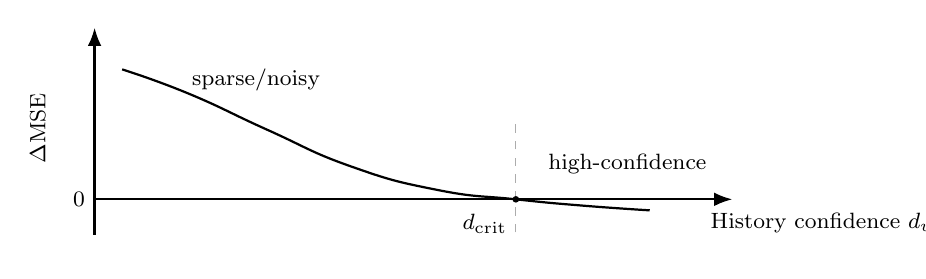
\begin{tikzpicture}[
    font=\footnotesize,
    axis/.style={-Latex,thick,black},
    guide/.style={dashed,gray!65},
    note/.style={align=center,inner sep=1pt,text=black},
]
    \path[use as bounding box] (-0.85,-0.65) rectangle (10.20,2.18);
    \draw[axis] (0,0) -- (8.10,0);
    \draw[axis] (0,-0.45) -- (0,2.18);
    \node[align=center,anchor=west,text=black] at (7.70,-0.30) {History confidence $d_v$};
    \node[align=center,rotate=90,text=black] at (-0.72,0.90)
        {$\Delta\mathrm{MSE}$};

    \node[left,text=black] at (0,0) {$0$};

    \draw[thick]
        plot[smooth,tension=0.85] coordinates {
            (0.35,1.65) (1.20,1.34) (2.20,0.88) (3.25,0.42)
            (4.35,0.12) (5.35,0.00) (6.20,-0.08) (7.05,-0.14)
        };

    \draw[guide] (5.35,-0.42) -- (5.35,1.05);
    \fill (5.35,0) circle (1.2pt);
    \node[note] at (2.05,1.52) {sparse/noisy};
    \node[note,anchor=west] at (5.72,0.45) {high-confidence};
    \node[note,anchor=north east] at (5.28,-0.15) {$d_{\mathrm{crit}}$};
\end{tikzpicture}
\captionof{figure}{Conceptual smoothing regime along a one-dimensional history-confidence scale. Here $\Delta_{\mathrm{MSE}}=\operatorname{MSE}(H)-\operatorname{MSE}(S_D)$. Positive values indicate an MSE reduction from smoothing. The schematic boundary $d_{\mathrm{crit}}$ marks the balance between the variance and squared-bias changes in Theorem~\ref{thm:mse-decomp}.}
\label{fig:regime-criterion}
\end{center}

The actual boundary in Figure~\ref{fig:regime-criterion} depends jointly on $L$, $D$, the latent risk $r$, the shrinkage bias $b_H$, and the noise covariance $\Sigma$. Corollary~\ref{cor:high-confidence} concerns squared-error risk, not ranking metrics directly. It nevertheless provides a regime guide for AUC-PR and $P@1\%$: sparse histories leave substantial estimation variance, whereas highly discriminative histories leave less residual information for a graph smoother to recover. In the latter case, neighborhood mismatch can alter an already accurate ordering.

\section{Scoring architecture}
\label{sec:architecture}

For a candidate transaction, let $a$ and $b$ denote the two entity nodes used by the selected risk relation (for example, a card and a device), and let $x$ collect the remaining transaction attributes. The adaptive field produces endpoint features such as
\[
    (\SD)_a,
    \quad
    (\SD)_b,
    \quad
    (\SD)_a+(\SD)_b,
    \quad
    \max\{(\SD)_a,(\SD)_b\},
    \quad
    |(\SD)_a-(\SD)_b|.
\]
With posterior uncertainty, the feature family can be expanded by $\sigma_a,\sigma_b$ and standardized risk terms.

The supervised tabular models use LightGBM gradient-boosted trees \cite{ke2017lightgbm}. We denote the causal tabular baseline by
\[
    M3=T+C+G+P,
\]
where $T$ contains transaction attributes available at scoring time, $C$ contains relation-specific cold-start, count, and recency features, $G$ contains graph aggregates such as weighted degrees and common-neighbor statistics, and $P$ contains temporal-link history. The released-history block $H_{\rm raw}$ applies the same endpoint and pair summaries to $H$ that are used above for $S_D$.

The non-adaptive ablation replaces nodewise confidence by a scalar fidelity parameter:
\[
    S_{\rm plain}=S_{\lambda}:=\lambda(L+\lambda I)^{-1}H,
    \qquad \lambda>0.
\]
Thus $S_{\rm plain}$ applies the same history fidelity at every node, whereas $S_D$ uses the exposure-dependent diagonal matrix $D$. The reported block-causal runs fix $\lambda=0.1$ before final test evaluation, and all model-selection choices use training and validation data only.

The alert-ranking models combine these causal feature blocks in two ways. Let $z_1,\ldots,z_m$ be validation-selected logits from candidate models using the baseline, raw-history, plain-Green, and adaptive-Green features. The Green-score ensemble is the nonnegative logit combination
\[
    z_{\rm soft}=\sum_{j=1}^m\omega_j z_j,
    \qquad \omega_j\ge0,
    \qquad \sum_{j=1}^m\omega_j=1.
\]
The implementation searches unnormalized weights in $\{0,0.25,0.5,0.75,1\}^m\setminus\{0\}$, normalizes by their sum, and selects lexicographically by validation $P@1\%$, validation $P@0.5\%$, and validation AUC-PR. The Green tail reranker first selects a high-risk candidate fraction using validation data and then fits a logistic reranker within that region. If $q_i^{(0)}$ is the base score and $z_i$ is the vector of Green-risk and history features, the second-stage probability is
\[
    p_i^{(2)}=\ell\!\left(\beta_0+\beta_1q_i^{(0)}+\beta^\top z_i\right),
    \qquad
    \ell(u)=\frac{1}{1+e^{-u}}.
\]
Let $c$ be the base-risk cutoff fixed on validation data. The final online score is pointwise:
\[
 q_i^{\rm tail}=
 \begin{cases}
 \tfrac12 q_i^{(0)}, & q_i^{(0)}<c,\\[2pt]
 \tfrac12+\tfrac12p_i^{(2)}, & q_i^{(0)}\ge c.
 \end{cases}
\]
Candidate fractions, $c$, and the logistic coefficients are chosen without test labels and then transferred unchanged to the test stream. Hence the score for transaction $i$ depends only on $\mathcal I_i$ and validation-frozen parameters; appending later test transactions cannot change an earlier score. The cross-fitted Green tail reranker uses chronological out-of-fold base scores on the training period before applying the same validation-stage selection. These outputs are ranking scores rather than calibrated probabilities, and calibration is assessed separately. Earlier test-batch-quantile/rank scores are retained only as pre-freeze diagnostics and are excluded from the final tables.

\section{Experimental protocol}
\label{sec:protocol}

The real-data experiments use the IEEE-CIS transaction data \cite{ieeecis}. The main evaluation uses five chronological 100k windows:
\[
    0\text{--}100k,
    \quad 100k\text{--}200k,
    \quad 200k\text{--}300k,
    \quad 300k\text{--}400k,
    \quad 400k\text{--}500k.
\]
Each window is split chronologically into $60k$ train, $20k$ validation, and $20k$ test. Model selection uses train and validation data only, and the test block is evaluated once. For the controlled headline experiment, graph and released-history state are reset at the start of each 100k window; a separate warm-start diagnostic below carries all earlier global chronology into each window. The main released-history estimate uses $\alpha=5$ in \eqref{eq:history}. Independently, the adaptive confidence uses $d_0=5$, giving $d_v=5+\sqrt{n_v}$.

The protocol uses timestamp-block causality. An implementation audit identified a same-timestamp ordering ambiguity: the candidate transaction itself was excluded and train/validation/test separation was intact, while earlier rows with the same observed \texttt{TransactionDT} could update the graph before later rows with that same timestamp. Because IEEE-CIS does not specify within-timestamp order, the final implementation uses the conservative block rule
\[
    B_t=\{i:\operatorname{TransactionDT}_i=t\}.
\]
All rows in $B_t$ are scored against the same frozen $t^-$ state built from earlier timestamps. Labels are available only if their release time is strictly less than the candidate timestamp. After all rows in $B_t$ are scored, the block is committed to the graph and its labels are scheduled for later release. All reported public-data results use this block-causal protocol.

For each candidate transaction, the implementation extracts a radius-2/cap-100 local ego graph around the candidate endpoints and solves the adaptive Green system exactly on that capped local graph. The cap is a total-node cap, including the two candidate endpoints; if the breadth-first expansion would exceed 100 nodes, the retained induced node set is sorted deterministically before matrix assembly. At this scale, dense assembly and Cholesky factorization remain computationally modest. The plain Green field fixes $\lambda=0.1$ before final test evaluation.

The reported base LightGBM fits use at most 700 trees, learning rate 0.04, column subsampling 0.9, training-prevalence class weighting, and early stopping after 50 validation rounds on average precision. The code sets a row subsample fraction of 0.9 but leaves the LightGBM subsample frequency at zero, so stochastic row bagging is not active in the frozen runs. Validation selects lexicographically by $P@1\%$, $P@0.5\%$, $P@2\%$, and AUC-PR from
\[
\begin{split}
(\text{leaves},\text{minimum child},\ell_2)\in\{&
(15,40,2),(31,20,1),\\
&(63,30,3),(31,80,5)\}.
\end{split}
\]
Tail rerankers use candidate fractions $\{2.5,5,10,20,30\}\%$ selected lexicographically by validation $P@1\%$, validation $P@0.5\%$, and validation AUC-PR. Logistic rerankers use balanced class weights, $C=0.5$, and at most 2000 iterations. The cross-fitted reranker uses three chronological out-of-fold blocks after a 50\% warm-up period; its fixed OOF base fits use at most 160 trees, learning rate 0.04, 31 leaves, minimum child size 40, $\ell_2=3$, and early stopping after 25 rounds.

For reproducibility, the public repository includes a machine-readable manifest containing the relation definitions, ego-graph truncation rule, model hyperparameters, calibration settings, random seeds, data-split identifiers, and hashes of the result summaries used to generate the tables and figures. These settings were fixed using training and validation data before final test evaluation.

Evaluation focuses on ranking and fixed alert budgets. The primary ranking metric is AUC-PR, the area under the precision--recall curve, which is standard for highly imbalanced rare-event problems \cite{davis2006relationship,saito2015precision}. The primary operational metric is precision at a fixed alert budget, especially $P@1\%$. For a score $q_i$, let $A_\rho$ be the set of transactions in the top $\rho$ fraction by score. Then
\[
    P@\rho=\frac{\sum_{i\in A_\rho}Y_i}{|A_\rho|}.
\]
The tables report mean gains across chronological windows. A win count such as $4/5$ means that the gain is positive in four of the five test windows.
Tree ensembles can assign identical scores to multiple transactions at an alert cutoff. All final alert-budget metrics therefore break ties deterministically by chronological arrival order using a stable sort. This policy is applied consistently during validation selection, test evaluation, placebo evaluation, and bootstrap resampling.


\section{Block-causal evaluation}
\label{sec:results}

Unless stated otherwise, the IEEE-CIS results use the five chronological 100k windows and the $60k/20k/20k$ train/validation/test split described above. Model selection used train and validation data only; test labels were not used for tuning. The causal-feature audit covered the base features, plain Green features, and adaptive-precision features used in the graph-history and delay experiments. The local Green features use exact dense radius-2/cap-100 ego-graph solves.

The first evaluation separates released-history effects from graph-propagation effects. Table~\ref{tab:global-m3} reports global gains over the causal $M3=T+C+G+P$ baseline. Raw released history contributes substantial signal. The confidence-weighted Green field adds a further graph-dependent increment in the immediate-release benchmark, while the delay sweep below shows how this standalone marginal changes as labels are withheld for longer periods.

\begin{table}[h]
\centering
\caption{Block-causal global gains over $M3$ across five chronological 100k windows.}
\label{tab:global-m3}
\resizebox{\linewidth}{!}{%
\begin{tabular}{lcccc}
\toprule
Model & Mean $\Delta$ AUC-PR & AUC wins & Mean $\Delta P@1\%$ & $P@1\%$ wins \\
\midrule
$M3+H_{\rm raw}$ & +0.0825 & 5/5 & +0.160 & 5/5 \\
$M3+H_{\rm raw}+S_D$ & +0.1027 & 5/5 & +0.240 & 5/5 \\
Green-score ensemble & +0.1250 & 5/5 & +0.323 & 5/5 \\
Green tail reranker & +0.1714 & 5/5 & \textbf{+0.426} & 5/5 \\
Cross-fitted Green tail reranker & \textbf{+0.1735} & 5/5 & +0.420 & 5/5 \\
\bottomrule
\end{tabular}}

{\footnotesize\emph{Note:} Gains are computed from unrounded window-level values; displayed rounded components therefore need not add exactly.}
\end{table}

Table~\ref{tab:history-marginal} isolates the graph marginal over raw released history in the immediate-release benchmark. Under timestamp-block causality, $M3+H_{\rm raw}+S_D$ improves over $M3+H_{\rm raw}$ by $+0.0202$ mean AUC-PR and $+0.080$ mean $P@1\%$. The AUC-PR marginal is positive in three windows, while the alert-budget marginal is positive in all five; the evidence is therefore stronger for top-budget ranking than for uniformly stable global ranking.

\begin{table}[h]
\centering
\caption{Graph marginal over raw released history under timestamp-block causality.}
\label{tab:history-marginal}
\resizebox{\linewidth}{!}{%
\begin{tabular}{lcccc}
\toprule
Comparison & Mean $\Delta$ AUC-PR & AUC wins & Mean $\Delta P@1\%$ & $P@1\%$ wins \\
\midrule
$M3+H_{\rm raw}+S_D$ vs. $M3+H_{\rm raw}$ & +0.0202 & 3/5 & +0.080 & 5/5 \\
Green tail reranker vs. $M3+H_{\rm raw}$ & +0.0889 & 5/5 & \textbf{+0.266} & 5/5 \\
Cross-fitted Green tail reranker vs. $M3+H_{\rm raw}$ & \textbf{+0.0910} & 5/5 & +0.260 & 5/5 \\
\bottomrule
\end{tabular}}
\end{table}

Table~\ref{tab:cohorts} breaks the graph-history effect into two deployment-relevant cohorts. The known-endpoint cohort contains transactions whose selected risk-layer endpoints have appeared before scoring. The new-pair cohort ($C00_{\rm newedge}$) is the cold/new-edge slice used in the audit: the selected endpoint pair is new at scoring time and the local released-history signal is weakest.

\begin{table}[h]
\centering
\caption{Critical-cohort gains over raw released history.}
\label{tab:cohorts}
\resizebox{\linewidth}{!}{%
\begin{tabular}{llcccc}
\toprule
Cohort & Model & Mean $\Delta$ AUC-PR & AUC wins & Mean $\Delta P@1\%$ & $P@1\%$ wins \\
\midrule
Known endpoints & $M3+H_{\rm raw}+S_D$ & +0.0192 & 3/5 & +0.0725 & 4/5 \\
Known endpoints & Green tail reranker & +0.0908 & 5/5 & +0.2670 & 5/5 \\
Known endpoints & Cross-fitted Green tail reranker & +0.0935 & 5/5 & +0.2649 & 5/5 \\
New pair & $M3+H_{\rm raw}+S_D$ & +0.0281 & 5/5 & +0.0277 & 3/5 \\
New pair & Green tail reranker & +0.1114 & 5/5 & +0.2378 & 5/5 \\
New pair & Cross-fitted Green tail reranker & +0.1152 & 5/5 & +0.2255 & 4/5 \\
\bottomrule
\end{tabular}}
\end{table}
\FloatBarrier

The standalone graph marginal is positive on average in both controlled cohorts. In the harder new-pair cohort, direct graph smoothing is AUC-positive in all five windows but its top-$1\%$ gain is less stable; the learned tail models recover larger gains on both metrics.

The tables report mean-over-window gains and window win counts. We also ran a paired chronological-block bootstrap over the pooled test transactions, using 500-row chronological blocks within each window and 2000 bootstrap replicates. The block size is a local-dependence sensitivity choice: it is large enough to preserve short bursts of temporally adjacent transactions while leaving multiple resampling blocks in each 20k-row test segment. Intervals are percentile intervals using the 2.5\% and 97.5\% bootstrap quantiles. These intervals check whether the paired ranking differences persist under local chronological resampling. Their point estimates are computed on pooled test transactions and therefore need not equal the unweighted mean of the five window-level gains reported in Tables~\ref{tab:global-m3}--\ref{tab:cohorts}.

\begin{table}[h]
\centering
\caption{Paired chronological-block bootstrap confidence intervals over pooled test transactions.}
\label{tab:bootstrap-ci}
\resizebox{\linewidth}{!}{%
\begin{tabular}{llrrrr}
\toprule
Cohort & Comparison & AUC-PR $\Delta$ & 95\% CI & $P@1\%$ $\Delta$ & 95\% CI \\
\midrule
All & $M3+H_{\rm raw}+S_D$ vs. $M3+H_{\rm raw}$ & +0.0439 & $[+0.0248,+0.0624]$ & +0.122 & $[+0.064,+0.171]$ \\
All & Green tail reranker vs. $M3$ & +0.1767 & $[+0.1546,+0.1985]$ & +0.510 & $[+0.452,+0.574]$ \\
All & Cross-fitted Green tail reranker vs. $M3$ & +0.1705 & $[+0.1469,+0.1919]$ & +0.505 & $[+0.442,+0.564]$ \\
Known endpoints & $M3+H_{\rm raw}+S_D$ vs. $M3+H_{\rm raw}$ & +0.0434 & $[+0.0261,+0.0620]$ & +0.1134 & $[+0.0557,+0.1662]$ \\
New pair & $M3+H_{\rm raw}+S_D$ vs. $M3+H_{\rm raw}$ & +0.0560 & $[+0.0270,+0.0873]$ & +0.1324 & $[+0.0146,+0.2279]$ \\
\bottomrule
\end{tabular}}
\end{table}

Bootstrap intervals are positive for the global, known-endpoint, and new-pair graph marginals and for the tail-ranking gains. These pooled estimates weight transactions rather than windows equally, so they need not reproduce the win counts in Table~\ref{tab:cohorts}.

The delay sweep changes the release schedule while leaving the chronological graph construction fixed. IEEE-CIS \texttt{TransactionDT} is measured in seconds, and the simulated delay $\delta$ is measured in days. Thus the release time is set to $\rho_i=\tau_i+86400\,\delta$, and a label is eligible only when $\rho_i<t$. Even for $\delta=0$, same-timestamp labels are not eligible because the block-causal rule releases labels only before the next strictly later timestamp block. The reported grid is $\delta\in\{0,1,3,7,14\}$. Table~\ref{tab:delay-static} reports the graph marginal over raw history under these schedules. The static marginal is largest at zero delay and attenuates as labels become less immediate.

\begin{table}[h]
\centering
\caption{Static graph marginal over raw history by label-release delay.}
\label{tab:delay-static}
\begin{tabular}{rcccc}
\toprule
$\delta$ & AUC-PR gain & AUC wins & $P@1\%$ gain & $P@1\%$ wins \\
\midrule
0 & +0.0202 & 3/5 & +0.080 & 5/5 \\
1 & -0.0210 & 1/5 & -0.051 & 2/5 \\
3 & +0.0164 & 3/5 & +0.057 & 4/5 \\
7 & -0.0059 & 2/5 & -0.019 & 1/5 \\
14 & +0.0060 & 4/5 & +0.022 & 1/5 \\
\bottomrule
\end{tabular}
\end{table}

The tail-ranking model is more stable across delays. Table~\ref{tab:delay-tail} and Figure~\ref{fig:delay-sweep} show that both the Green tail reranker and the cross-fitted Green tail reranker improve over raw history across all tested delays. The five 100k windows span 22.2, 29.5, 33.1, 31.0, and 35.0 days, respectively; their 20k-row test segments span 3.3--7.6 days. Longer 30- and 60-day chargeback delays therefore require longer chronological windows than this protocol provides.

\begin{table}[h]
\centering
\caption{Tail-reranker gains over raw history by label-release delay.}
\label{tab:delay-tail}
\resizebox{\linewidth}{!}{%
\begin{tabular}{rlcccc}
\toprule
$\delta$ & Model & AUC-PR gain & AUC wins & $P@1\%$ gain & $P@1\%$ wins \\
\midrule
0 & Green tail reranker & +0.0889 & 5/5 & +0.266 & 5/5 \\
1 & Green tail reranker & +0.0430 & 4/5 & +0.140 & 5/5 \\
3 & Green tail reranker & +0.0641 & 5/5 & +0.209 & 5/5 \\
7 & Green tail reranker & +0.0596 & 5/5 & +0.196 & 5/5 \\
14 & Green tail reranker & +0.0671 & 5/5 & +0.173 & 5/5 \\
0 & Cross-fitted Green tail reranker & +0.0910 & 5/5 & +0.260 & 5/5 \\
1 & Cross-fitted Green tail reranker & +0.0421 & 4/5 & +0.141 & 5/5 \\
3 & Cross-fitted Green tail reranker & +0.0656 & 5/5 & +0.238 & 5/5 \\
7 & Cross-fitted Green tail reranker & +0.0613 & 5/5 & +0.217 & 5/5 \\
14 & Cross-fitted Green tail reranker & +0.0395 & 5/5 & +0.190 & 4/5 \\
\bottomrule
\end{tabular}}
\end{table}

\begin{center}
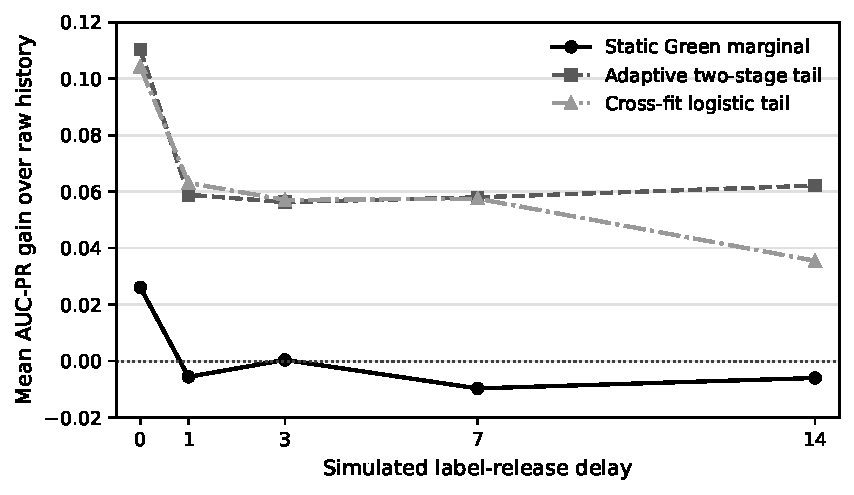
\includegraphics[width=0.78\linewidth]{../figures/fig_delay_auc_sweep.pdf}
\captionof{figure}{Delay sweep for AUC-PR gains over raw released history on IEEE-CIS. The standalone Green marginal is largest under immediate release and attenuates under delayed labels. Tail-ranking models using Green-risk features remain positive across all tested delays.}
\label{fig:delay-sweep}
\end{center}

The contrast indicates that the delay-stable contribution arises primarily from the interaction of Green-risk features with the tail-ranking model, rather than from standalone smoothing.

Table~\ref{tab:audit} summarizes the leakage and causality audit. It checks future-edge exclusion, candidate self-exclusion, label-release order, same-timestamp block policy, train/validation/test separation, and cache provenance. The same-timestamp case is nontrivial: across the five windows, 29,694 rows had tied timestamps and 3,642 rows shared risk-layer endpoints inside tied timestamps. Final scoring excludes all same-timestamp influence by construction.

\begin{table}[h]
\centering
\caption{Block-causal leakage audit. A PASS indicates that the corresponding executable assertion held for every audited scoring block.}
\label{tab:audit}
\resizebox{\linewidth}{!}{%
\begin{tabular}{lll}
\toprule
Check & Verification criterion & Status \\
\midrule
Future-edge exclusion & every feature edge has insertion time $<t$ & PASS \\
Candidate self-exclusion & candidate-generated edges are absent at scoring & PASS \\
Label-release audit & every history label satisfies $\rho_i<t$ & PASS \\
Same-timestamp policy & all rows in $B_t$ use one frozen $t^-$ state & PASS \\
Train/validation/test separation & fitting and selection exclude test labels & PASS \\
Cached feature provenance & cache keys identify data split, delay, and configuration & PASS \\
Pointwise tail scoring & appending later test rows leaves earlier scores unchanged & PASS \\
Alert-score ties & stable chronological tie policy is used in selection and evaluation & PASS \\
\bottomrule
\end{tabular}}
\end{table}

The permutation placebo is a negative control. Released-history labels used to construct $H_{\rm raw}$, $S_D$, and tail meta-features were permuted within each chronological window, while graph structure, timestamps, splits, and evaluation labels were left unchanged. Table~\ref{tab:placebo} shows that the released-history and graph gains are largely removed under permutation.

\begin{table}[h]
\centering
\caption{Permutation placebo. Real gains use true released-history labels; placebo gains permute released-history labels while keeping graph structure and evaluation labels fixed.}
\label{tab:placebo}
\resizebox{\linewidth}{!}{%
\begin{tabular}{lrrrr}
\toprule
Comparison & Real AUC gain & Placebo AUC gain & Real $P@1\%$ gain & Placebo $P@1\%$ gain \\
\midrule
$M3+H_{\rm raw}$ vs. $M3$ & +0.0825 & -0.0045 & +0.160 & +0.022 \\
$M3+H_{\rm raw}+S_D$ vs. $M3$ & +0.1027 & -0.0033 & +0.240 & +0.013 \\
$M3+H_{\rm raw}+S_D$ vs. $M3+H_{\rm raw}$ & +0.0202 & +0.0012 & +0.080 & -0.009 \\
Green-score ensemble vs. $M3$ & +0.1250 & +0.0080 & +0.323 & +0.036 \\
Green tail reranker vs. $M3$ & +0.1714 & +0.0387 & +0.426 & +0.150 \\
Green tail reranker vs. $M3+H_{\rm raw}$ & +0.0889 & +0.0432 & +0.266 & +0.128 \\
\bottomrule
\end{tabular}}
\end{table}

The graph marginal $M3+H_{\rm raw}+S_D$ over $M3+H_{\rm raw}$ is sharply weakened under permutation, changing from $+0.0202$ to $+0.0012$ AUC-PR and from $+0.080$ to $-0.009$ $P@1\%$. This pattern shows that the graph marginal depends on the association between released labels and the historical graph, rather than on graph structure alone. The residual positive tail gain under permutation is also much smaller and is consistent with the tail model retaining non-history baseline risk.

Calibration is evaluated separately from alert ranking. Table~\ref{tab:calibration} reports the Brier score, the mean squared error of the predicted probabilities, and ECE, the expected calibration error computed with 10 equal-frequency bins in each test window. The model $M3+H_{\rm raw}+S_D$ has the lowest Brier score among the four evaluated probability scores. The Green tail-reranker score is overconfident in the top tail and is therefore reported as an alert-ranking score, with probability calibration left to the graph-history model.

\begin{table}[h]
\centering
\caption{Mean calibration diagnostics over five block-causal windows.}
\label{tab:calibration}
\resizebox{\linewidth}{!}{%
\begin{tabular}{lrrrrr}
\toprule
Model & Mean score & Brier & ECE & Top-1\% observed & Top-1\% mean score \\
\midrule
$M3$ & 0.0513 & 0.0338 & 0.0285 & 0.157 & 0.0910 \\
$M3+H_{\rm raw}$ & 0.0570 & 0.0331 & 0.0365 & 0.317 & 0.1205 \\
$M3+H_{\rm raw}+S_D$ & 0.0562 & \textbf{0.0329} & 0.0340 & 0.397 & 0.1290 \\
Green tail reranker & 0.1760 & 0.1141 & 0.1442 & \textbf{0.583} & 0.9584 \\
\bottomrule
\end{tabular}}
\end{table}

Among the evaluated probability-score models, the graph-history model has the lowest Brier score and a higher observed fraud concentration in the top tail. The two-stage model gives the highest top-alert ranking performance; probabilistic use would require post-hoc calibration.

The GMRF interpretation suggests posterior-variance and standardized-risk features based on $\sigma_v^2=[(L+D)^{-1}]_{vv}$. A small pre-freeze diagnostic tested endpoint posterior variances and posterior $z$-scores, but it did not meet the prespecified requirement to replace the corrected five-window headline in at least four windows. Because that diagnostic predates the final stable-tie model freeze, its numerical table is not mixed with the final results; posterior uncertainty is left as future work rather than promoted through additional tuning.

The benchmark protocol resets graph/history state at the beginning of each 100k window, which creates artificial cold starts. A warm-started diagnostic lets each scored window inherit graph/history state from all earlier rows in the global chronology while preserving timestamp-block scoring, closer to a continuously running deployment. In that diagnostic, $M3+H_{\rm raw}+S_D$ exceeds $M3+H_{\rm raw}$ by $+0.0161$ mean AUC-PR (4/5 windows) and $+0.050$ mean $P@1\%$ (3/5 windows). The graph marginal therefore survives continuous-state evaluation but is weaker and less top-tail-stable than in the reset-window benchmark. An earlier warm-start tail diagnostic used a whole-test-batch rank transformation and is excluded from the final claims; the pointwise validation-threshold score in the main results removes that dependence directly.

\section{Discussion}

The empirical results are consistent with the estimator's bias--variance structure. IEEE-CIS is not uniformly cold, but it contains many weak-link and new-pair cases. Across the five test segments, 13.7\% of scored rows are in the new-pair cohort; 31.5\% have weakest released endpoint count at most 20 across the selected Green-risk layers; and 4.5\% have at least one zero-count released endpoint. In this regime, $M3+H_{\rm raw}+S_D$ improves over $M3+H_{\rm raw}$ on mean AUC-PR and in all five $P@1\%$ comparisons under timestamp-block processing. Paired block-bootstrap intervals are positive globally and in both controlled cohorts, while released-label permutation sharply weakens the marginal gain. The Green tail reranker gives the highest mean top-alert precision, while $M3+H_{\rm raw}+S_D$ has the lowest Brier score among the evaluated probability-score models.

Elliptic++ provides a case on the saturated operating-budget side of the same conceptual boundary. Released address history is already highly informative at the top alert budget, where the raw-history baseline reaches $P@1\%=1.00$, leaving little residual top-tail signal for a graph smoother to recover. In that setting exact local Green fields perform below the strongest raw-history baseline. Across the two datasets, the value of smoothing depends on local-history uncertainty, neighborhood smoothness, and the remaining headroom at the alert budget.

\section{Limitations}

The empirical validation has bounded scope. IEEE-CIS is anonymized and attribute-derived, making the graph a public benchmark proxy for a production card--merchant--device network. The five 100k chronological windows provide an auditable public-data protocol spanning 22.2--35.0 days per window; longer 30/60-day chargeback horizons require longer chronological windows. The standalone graph marginal is positive in only 3/5 AUC-PR window comparisons, despite 5/5 $P@1\%$ gains, and the new-pair-cohort top-$1\%$ graph-only effect is less stable because very few alerts determine that metric. Resetting state at each 100k boundary also overstates cold-start prevalence relative to continuous deployment; the warm-start diagnostic remains positive but weaker.

A matched temporal-GNN benchmark would require the same timestamp-block graph snapshots, released-label schedule, and validation-only model selection, so that differences reflect architecture rather than information availability. The experiments here isolate the question addressed by the theory: the marginal value of an auditable Green layer beyond raw released history. Posterior-uncertainty features add a small diagnostic signal, and the Elliptic++ appendix supplies an external operating-budget saturation case.

\section{Conclusion}

Adaptive Green risk fields propagate released fraud history through a dynamic graph without using future edges or unreleased labels. The estimator
\[
        S_D=(L+D)^{-1}DH
\]
combines graph smoothing with nodewise confidence, admits variational and GMRF interpretations, and has an MSE decomposition that explicitly includes the bias of the shrinkage history estimator. The IEEE-CIS experiments show that the standalone graph marginal over raw released history is largest under immediate release and attenuates as labels are delayed. The delay-stable operational effect is tail ranking: models using Green-risk features improve over raw history across all tested release delays. Leakage audits and label-permutation placebos assess temporal validity and signal provenance, while bootstrap intervals and delay sweeps assess stability. Calibration diagnostics distinguish probability quality from alert-ranking performance. Elliptic++ supplies a complementary operating-budget saturation case: when raw address history is already highly discriminative at the alert budget, additional smoothing has little residual signal to exploit. Together these results give a causal released-history methodology, an interpretable Green smoothing layer, and a regime criterion for graph smoothing in fraud ranking.


\section*{Data availability}
The experiments use public benchmark datasets: IEEE-CIS Fraud Detection and Elliptic++. No proprietary transaction records are used in this manuscript. Derived result summaries are available from the author upon reasonable request.

\section*{Code availability}
The experimental implementation and result-generation scripts are available at \url{https://github.com/MaKosmakov/green-fraud-fields}. The repository contains the implementation, experiment manifest, tests, and scripts used to regenerate the reported tables and figures. Generated experiment outputs are not redistributed; processed summaries are available from the author upon reasonable request.

\section*{Funding}
This research received no specific grant from any funding agency in the public, commercial, or not-for-profit sectors.

\section*{Declaration of competing interest}
The author declares that there are no known competing financial interests or personal relationships that could have appeared to influence the work reported in this paper.

\section*{Declaration of generative AI and AI-assisted technologies}
During the preparation of this work, AI-assisted tools were used for language editing and manuscript organization. The author reviewed and edited the content and takes full responsibility for the manuscript.

\appendix
\section{External Elliptic++ regime check}
\label{app:ellipticpp}

Elliptic++ provides an external case for the regime analysis \cite{elmougy2023}. This check used temporal time-step blocks: all transactions in a time step were scored before labels from that block could update released address history, official wallet labels were excluded from features, unknown class-3 transactions were excluded from training and evaluation, and aggregate transaction features were excluded to preserve causality. The goal was to examine the released-history construction and local Green smoothing in a different temporal financial graph.

The result is consistent with the regime picture from Theorem~\ref{thm:mse-decomp} and Corollary~\ref{cor:high-confidence}. Raw released address history improves over strict transaction features and already reaches $P@1\%=1.000$. This is a saturated top-tail operating regime: little residual signal remains for smoothing at the alert budget, and graph mismatch can perturb an accurate ranking. Exact local Green smoothing on the current address graph falls below the strongest raw-history baseline. Table~\ref{tab:ellipticpp-smoke} summarizes the diagnostic.

\begin{table}[h]
\centering
\caption{Elliptic++ strict time-block regime check. Raw causal address history is saturated at the top alert budget; exact local Green variants remain below it.}
\label{tab:ellipticpp-smoke}
\begin{tabular}{lcc}
\toprule
Model & AUC-PR & $P@1\%$ \\
\midrule
Strict transaction features & 0.5976 & 0.970 \\
$H_{\rm raw}$, $\alpha=5$ & \textbf{0.6299} & \textbf{1.000} \\
$H_5+S_D$, radius 1, cap 50, $\alpha=5$ & 0.6058 & 0.960 \\
$H_5+S_D$, radius 2, cap 50, $\alpha=5$ & 0.6012 & 0.930 \\
$H_5+S_D$, radius 1, cap 50, $\alpha=20$ & 0.6088 & 0.970 \\
\bottomrule
\end{tabular}
\end{table}

Elliptic++ provides an external example consistent with operating-budget saturation: released address history saturates the top alert budget, and the tested local Green variants do not improve on that baseline. The same condition appears in the MSE decomposition: graph smoothing is most useful when local histories are sparse or noisy relative to graph smoothness, and least useful when released history is already highly discriminative at the operating budget.

\begin{thebibliography}{99}

\bibitem{ieeecis}
IEEE Computational Intelligence Society.
IEEE-CIS Fraud Detection dataset. Kaggle competition, 2019.

\bibitem{zhu2003}
X. Zhu, Z. Ghahramani, and J. Lafferty.
Semi-supervised learning using Gaussian fields and harmonic functions.
In \emph{Proceedings of the 20th International Conference on Machine Learning (ICML)}, 2003.

\bibitem{zhou2004}
D. Zhou, O. Bousquet, T. N. Lal, J. Weston, and B. Schölkopf.
Learning with local and global consistency.
In \emph{Advances in Neural Information Processing Systems (NeurIPS)}, 2004.

\bibitem{belkin2006}
M. Belkin, P. Niyogi, and V. Sindhwani.
Manifold regularization: a geometric framework for learning from labeled and unlabeled examples.
\emph{Journal of Machine Learning Research}, 7:2399--2434, 2006.

\bibitem{smola2003}
A. J. Smola and R. Kondor.
Kernels and regularization on graphs.
In \emph{Learning Theory and Kernel Machines}, Lecture Notes in Computer Science 2777, pages 144--158. Springer, 2003.

\bibitem{chapelle2006}
O. Chapelle, B. Schölkopf, and A. Zien, editors.
\emph{Semi-Supervised Learning}.
MIT Press, 2006.

\bibitem{rueheld}
H. Rue and L. Held.
\emph{Gaussian Markov Random Fields: Theory and Applications}.
Chapman and Hall/CRC, 2005.

\bibitem{chung1997}
F. R. K. Chung.
\emph{Spectral Graph Theory}.
CBMS Regional Conference Series in Mathematics, Vol. 92. American Mathematical Society, 1997.

\bibitem{rasmussen2006}
C. E. Rasmussen and C. K. I. Williams.
\emph{Gaussian Processes for Machine Learning}.
MIT Press, 2006.

\bibitem{shuman2013}
D. I. Shuman, S. K. Narang, P. Frossard, A. Ortega, and P. Vandergheynst.
The emerging field of signal processing on graphs: extending high-dimensional data analysis to networks and other irregular domains.
\emph{IEEE Signal Processing Magazine}, 30(3):83--98, 2013.

\bibitem{ortega2018}
A. Ortega, P. Frossard, J. Kovačević, J. M. F. Moura, and P. Vandergheynst.
Graph signal processing: overview, challenges, and applications.
\emph{Proceedings of the IEEE}, 106(5):808--828, 2018.

\bibitem{boltonhand2002}
R. J. Bolton and D. J. Hand.
Statistical fraud detection: a review.
\emph{Statistical Science}, 17(3):235--255, 2002.

\bibitem{phua2010}
C. Phua, V. Lee, K. Smith, and R. Gayler.
A comprehensive survey of data mining-based fraud detection research.
\emph{arXiv:1009.6119}, 2010.

\bibitem{akoglu2015}
L. Akoglu, H. Tong, and D. Koutra.
Graph based anomaly detection and description: a survey.
\emph{Data Mining and Knowledge Discovery}, 29:626--688, 2015.

\bibitem{ranshous2015}
S. Ranshous, S. Shen, D. Koutra, S. Harenberg, C. Faloutsos, and N. F. Samatova.
Anomaly detection in dynamic networks: a survey.
\emph{WIREs Computational Statistics}, 7(3):223--247, 2015.

\bibitem{weber2019}
M. Weber, G. Domeniconi, J. Chen, D. K. I. Weidele, C. Bellei, T. Robinson, and C. E. Leiserson.
Anti-money laundering in Bitcoin: experimenting with graph convolutional networks for financial forensics.
In \emph{KDD Workshop on Anomaly Detection in Finance}, 2019.

\bibitem{elmougy2023}
Y. Elmougy and L. Liu.
Demystifying fraudulent transactions and illicit nodes in the Bitcoin network for financial forensics.
\emph{arXiv:2306.06108}, 2023.

\bibitem{kipf2017}
T. N. Kipf and M. Welling.
Semi-supervised classification with graph convolutional networks.
In \emph{International Conference on Learning Representations (ICLR)}, 2017.

\bibitem{hamilton2017}
W. L. Hamilton, R. Ying, and J. Leskovec.
Inductive representation learning on large graphs.
In \emph{Advances in Neural Information Processing Systems (NeurIPS)}, 2017.

\bibitem{velickovic2018}
P. Veličković, G. Cucurull, A. Casanova, A. Romero, P. Liò, and Y. Bengio.
Graph attention networks.
In \emph{International Conference on Learning Representations (ICLR)}, 2018.

\bibitem{pareja2020}
A. Pareja, G. Domeniconi, J. Chen, T. Ma, T. Suzumura, H. Kanezashi, T. Kaler, C. E. Leiserson, and C. D. Schardl.
EvolveGCN: evolving graph convolutional networks for dynamic graphs.
In \emph{Proceedings of the AAAI Conference on Artificial Intelligence}, 2020.

\bibitem{sankar2020}
A. Sankar, Y. Wu, L. Gou, W. Zhang, and H. Yang.
DySAT: deep neural representation learning on dynamic graphs via self-attention networks.
In \emph{Proceedings of the 13th ACM International Conference on Web Search and Data Mining (WSDM)}, 2020.

\bibitem{xu2020}
D. Xu, C. Ruan, E. Körpeoglu, S. Kumar, and K. Achan.
Inductive representation learning on temporal graphs.
In \emph{International Conference on Learning Representations (ICLR)}, 2020.

\bibitem{rossi2020}
E. Rossi, B. Chamberlain, F. Frasca, D. Eynard, F. Monti, and M. Bronstein.
Temporal graph networks for deep learning on dynamic graphs.
\emph{arXiv:2006.10637}, 2020.

\bibitem{ke2017lightgbm}
G. Ke, Q. Meng, T. Finley, T. Wang, W. Chen, W. Ma, Q. Ye, and T.-Y. Liu.
LightGBM: a highly efficient gradient boosting decision tree.
In \emph{Advances in Neural Information Processing Systems (NeurIPS)}, 2017.

\bibitem{davis2006relationship}
J. Davis and M. Goadrich.
The relationship between precision-recall and ROC curves.
In \emph{Proceedings of the 23rd International Conference on Machine Learning (ICML)}, 2006.

\bibitem{saito2015precision}
T. Saito and M. Rehmsmeier.
The precision-recall plot is more informative than the ROC plot when evaluating binary classifiers on imbalanced datasets.
\emph{PLOS ONE}, 10(3):e0118432, 2015.

\bibitem{zadrozny2002}
B. Zadrozny and C. Elkan.
Transforming classifier scores into accurate multiclass probability estimates.
In \emph{Proceedings of the 8th ACM SIGKDD International Conference on Knowledge Discovery and Data Mining}, 2002.

\bibitem{niculescu2005}
A. Niculescu-Mizil and R. Caruana.
Predicting good probabilities with supervised learning.
In \emph{Proceedings of the 22nd International Conference on Machine Learning (ICML)}, 2005.

\bibitem{guo2017}
C. Guo, G. Pleiss, Y. Sun, and K. Q. Weinberger.
On calibration of modern neural networks.
In \emph{Proceedings of the 34th International Conference on Machine Learning (ICML)}, 2017.

\end{thebibliography}

\end{document}
